
\section{1.课程简介}

\begin{frame}
    \frametitle{课程内容}
        \begin{enumerate}
            \Item Fundamentals of quantum informatics(2学时)
            \IItem Fundamentals of quantum mechanics(2学时)
            \Item Quantum information processing and computing(8学时)
            \Item Quantum communication(8学时)
        \end{enumerate}
\end{frame}
\begin{frame} 
    \frametitle{分数构成}
        \begin{enumerate}
            \Item Normal results 20\%
            \Item Group discussion 30\%
            \Item Project final report 50\%
        \end{enumerate}
\end{frame}

\begin{frame}
    \frametitle{参考书目}
        \begin{itemize}
            \Item 《量子计算与量子信息》 (10周年版)  [美]Michael A. Nielsen,Isaac L. Chuang,清华大学出版社,2015        
            \Item 《量子信息处理技术》,赵生妹,郑宝玉,北京邮电大学出版社,2010
            \Item 《Quantum Computation and Quantum Information》(10th Anniversary Edition) , M. A. Nielsen, I. L. Chuang,Cambridge University Press,2011
            \Item 《Quantum Information, Computation and Communication》J. A. Jones,D. Jaksch,Oxford  University Press, 2012
            \Item 《量子信息物理原理》,科学出版社,张永德,   2016
        \end{itemize}
\end{frame}

\begin{frame}
    \begin{tcolorbox4}[分组讨论及报告专题设置(1)]    
        \begin{enumerate}
            \Item  量子叠加态的基本特性及其在量子信息处理中的应用;
            \Item  量子纠缠态的基本特性及其在量子通信中的应用;
            \Item  量子测量的基本特性及其在量子信息学中的应用;
            \Item  信息謪的香农定义和冯诺依曼定义及所带来的影响;
            \Item  量子加法器的量子门及光学线路;
            \Item  量子傅里叶变换的量子线路及光学实现;(明确傅里叶变换的量子基础,明确实现变换的光电器件及线路)
            \Item  质因数量子分解及破获经典密码的量子线路; 
            \Item   单光子、纠缠光子对的产生及检测技术;(该专题应深度结合光电专业知识和技术,明确其在量子信息领域的实际场景) 
        \end{enumerate}
    \end{tcolorbox4} 
\end{frame}

\begin{frame}
    \begin{tcolorbox4}[分组讨论及报告专题设置(2)]    
        \begin{enumerate}
            \Item   量子计算的物理模型与实现;
            \Item   BB84通信协议原理及光学实现;
            \Item   基于纠缠光子对的量子远程传态、量子密钥分配及实现方案;(基于光子技术,理解量子传态的原理,实现的光路及逻辑基础)
            \Item   拉曼散射光学量子中继原理及实现;
            \Item   压缩态的基本特性及其在量子信息学的应用;
            \Item  量子光学通信的研究前沿及最近进展
            \Item  自选专题
        \end{enumerate}
    \end{tcolorbox4} 
\end{frame}

%%%%%%%%%%%%%%%%%%%%%%%%%%%%%%%%%%%55%%
\begin{frame} [plain]
    \frametitle{}
    \Background[1] 
    \begin{center}
    {\huge 第1讲:量子信息与通信基础}
    \end{center}  
    \addtocounter{framenumber}{-1}   
\end{frame}
%%%%%%%%%%%%%%%%%%%%%%%%%%%%%%%%%%

\section{2.量子信息学简介}

\begin{frame} 
    \frametitle{量子信息学定义}
    量子信息学是基于量子力学基本原理对信息进行编码、存储、通信和计算处理的新兴交叉学科。Quantum information: Information that is acquired, processed, or transmitted by a system whose description requires quantum mechanics\\
    \begin{center}
        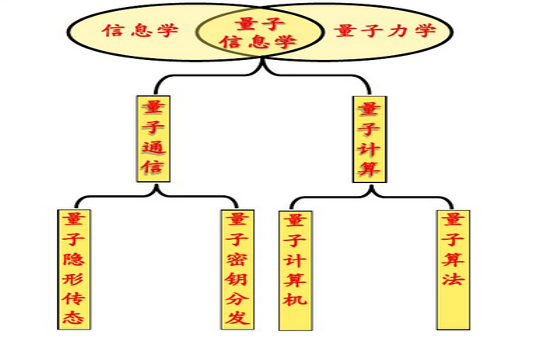
\includegraphics[width=0.55\textwidth]{figs/1.png}
    \end{center}   
\end{frame}

\begin{frame} 
    \frametitle{量子信息学应用}
    \begin{center}
        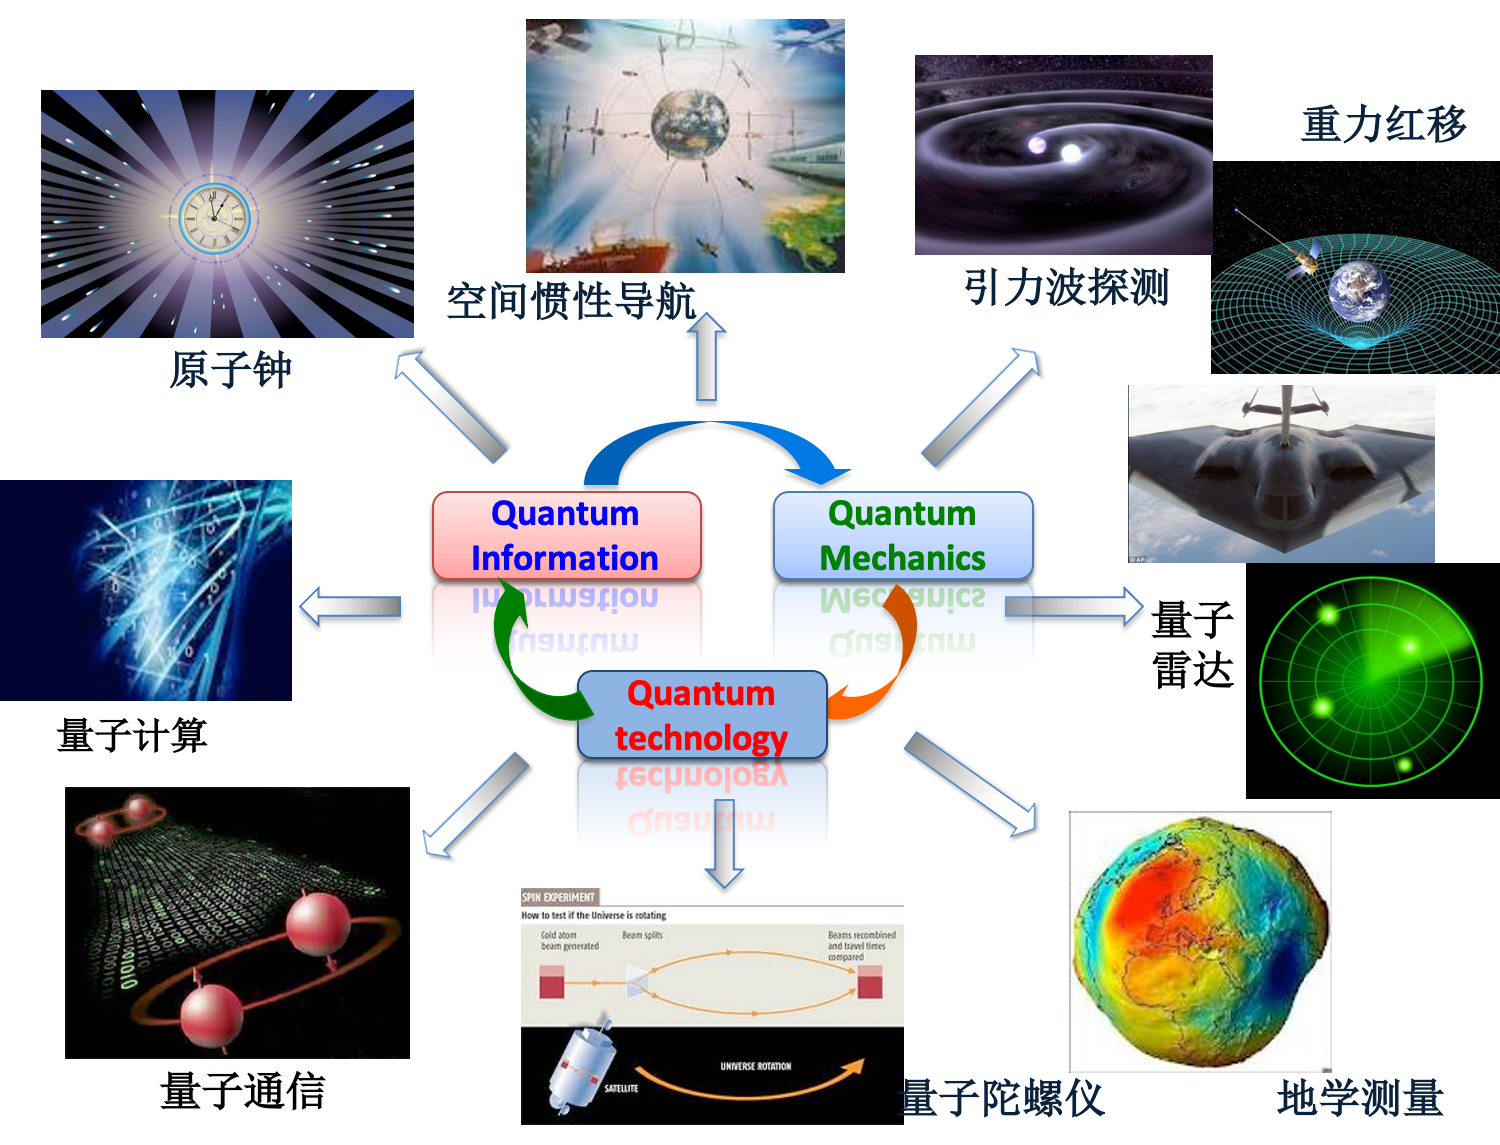
\includegraphics[width=0.7\textwidth]{figs/2.png}
    \end{center}   
\end{frame}

\begin{frame} 
    \frametitle{计算机发展简史}
    \begin{enumerate}
        \Item   算盘 (人力)
        \Item   图灵机(1930)机械,力学
        \Item   电子计算机(1946-1956)电学,真空-电子管,
        \Item   晶体管计算机(1956-1964) 数字,卡片机
        \Item   集成电路(1964-1970)单片机,磁盘,操作系统
        \Item   超大规模集成电路(1970-至今)微处理器
        \Item   量子计算机(...)
    \end{enumerate}
\end{frame}

\begin{frame} 
    \frametitle{Moor's Lore}
    \begin{center}
        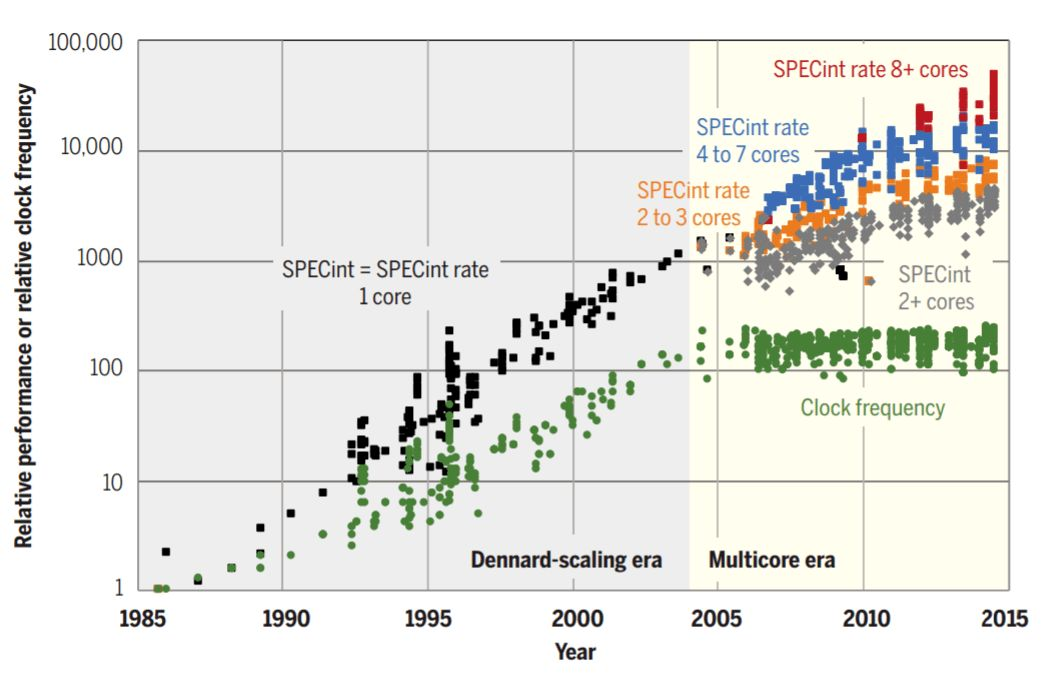
\includegraphics[width=0.8\textwidth]{figs/3.png}
    \end{center} 
\end{frame}

\begin{frame} 
    \frametitle{量子计算机的提出}
    \begin{center}
        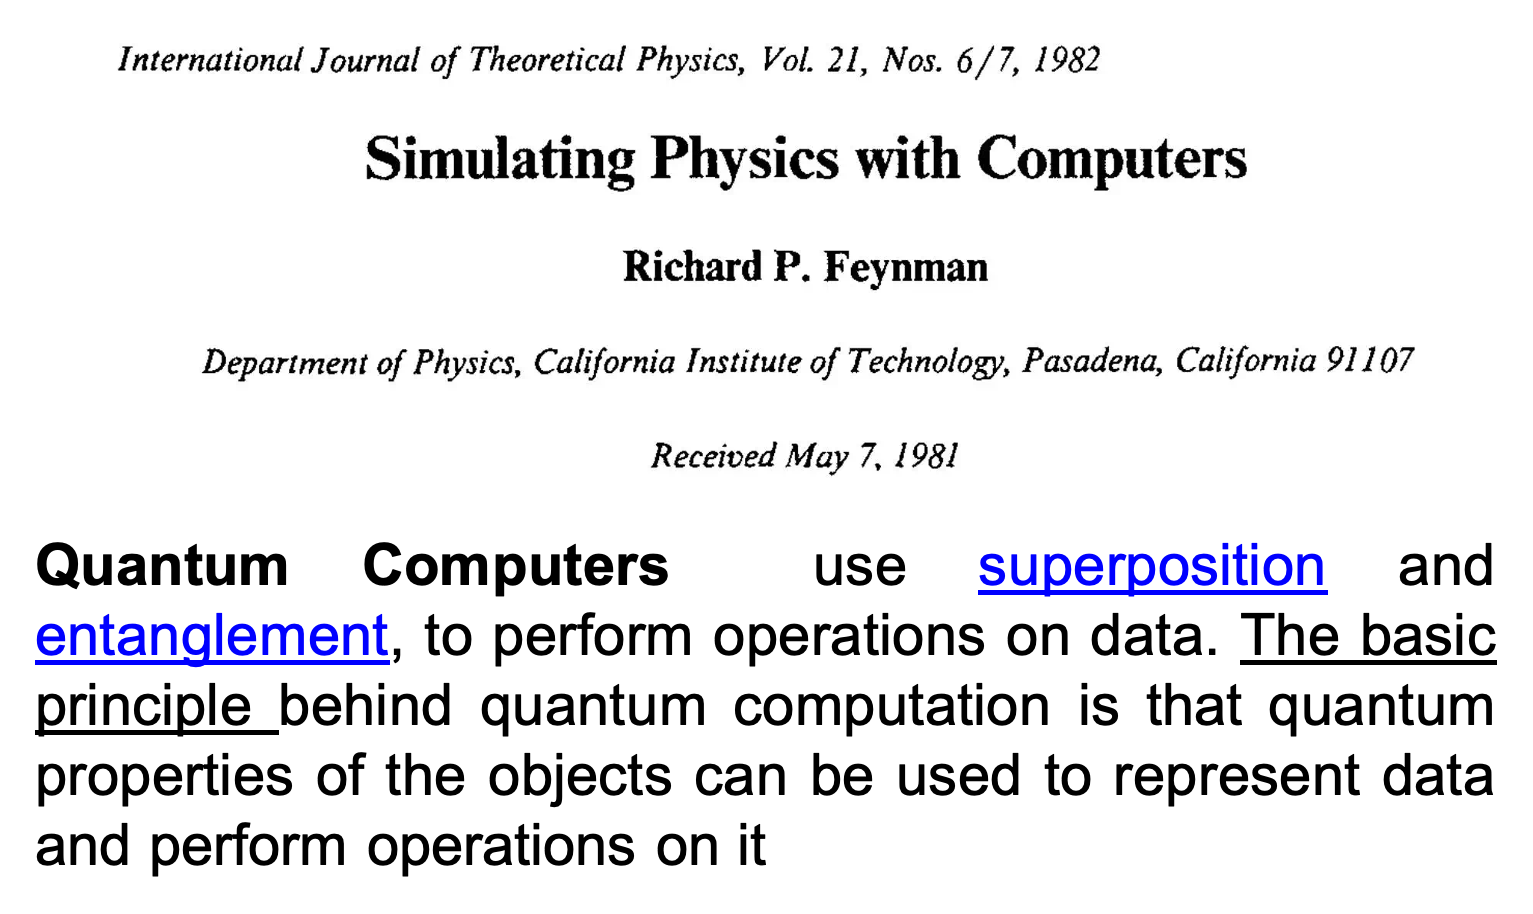
\includegraphics[width=0.8\textwidth]{figs/4.png}
    \end{center} 
\end{frame}

\begin{frame} 
    \frametitle{量子计算实现的难点}
    \begin{enumerate}
        \Item   量子计算机的顶层设计(数学模型)
        \Item   量子信息表示(比特与物理模型)
        \Item   量子态的保持(叠加态消相干)
        \Item   多量子并行(多量子多自由度纠缠)
    \end{enumerate}
\end{frame}

\begin{frame} 
    \frametitle{量子通信实现的难点}
    \begin{enumerate}
        \Item   量子态能传多远
        \Item   量子纠缠能传多远
    \end{enumerate}
    \begin{center}
        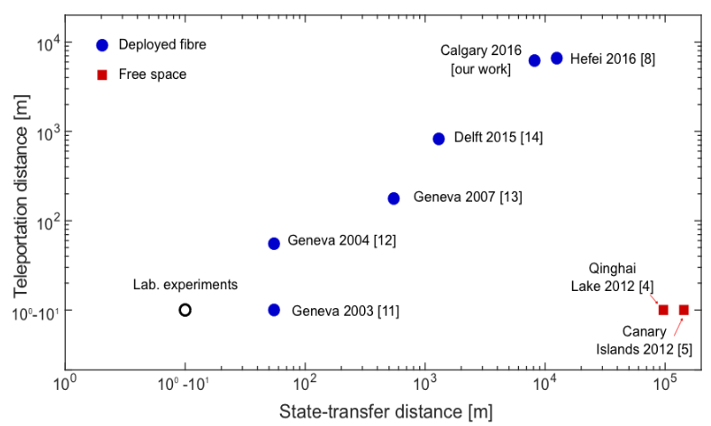
\includegraphics[width=0.6\textwidth]{figs/5.png}
    \end{center} 
\end{frame}

\begin{frame} 
    \frametitle{量子计算发展三阶段}
    \begin{center}
        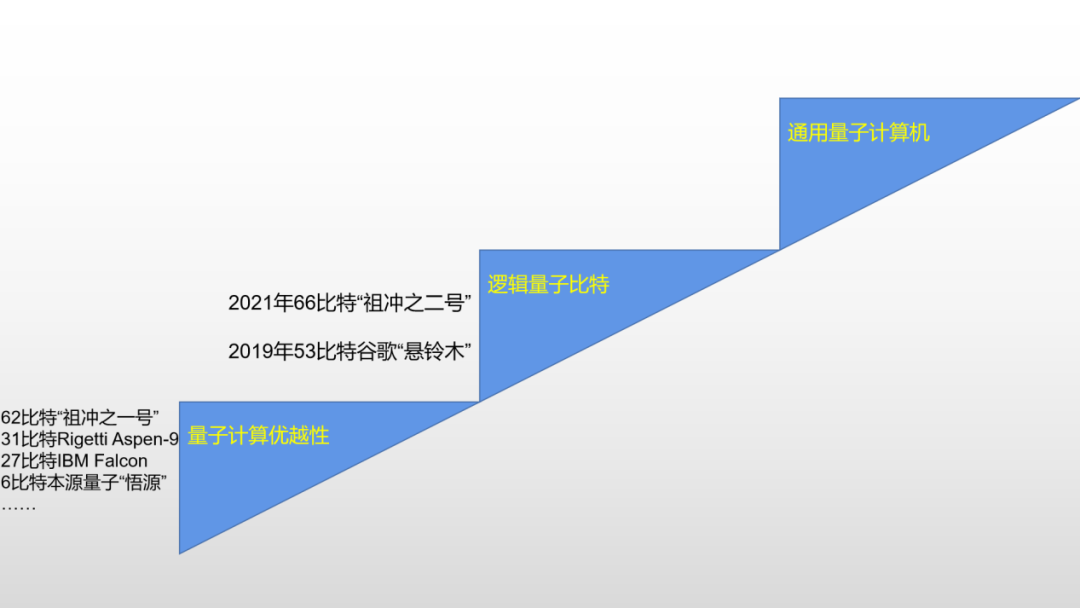
\includegraphics[width=0.9\textwidth]{figs/6.png}
    \end{center} 
\end{frame}

\begin{frame} 
    \frametitle{量子计算公司TOP10}
    \begin{enumerate}
        \Item   Accenture(埃森哲,英)
        \Item   阿里巴巴
        \Item   AT\&T
        \Item   Atos(源讯)
        \Item   百度
        \Item   谷歌
        \Item   IBM
        \Item   Intel
        \Item   微软
    \end{enumerate}
\end{frame}

\section{3.量子比特}

\begin{frame} 
    \frametitle{Bit and Qubit}
    \begin{center}
        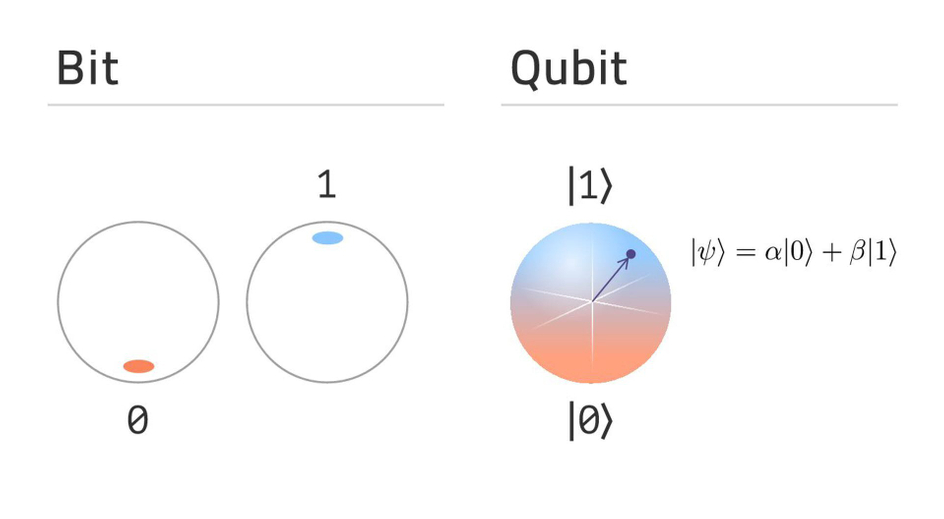
\includegraphics[width=0.8\textwidth]{figs/7.png}
    \end{center} 
\end{frame}

\begin{frame} 
    \frametitle{量子比特的物理实现}
    量子比特在物理上是二能级系统,因此,有以下可能的实现方案\\
    \begin{enumerate}
        \Item   光子
        \Item   电子
        \Item   原子
        \Item   离子色心
        \Item   分子
        \Item   超导材料
        \Item   拓扑材料
    \end{enumerate}
\end{frame}

\begin{frame} 
    \frametitle{量子比特的数学抽象}   
    这两个能态在数学上可抽象为
    \begin{enumerate}
        \Item   $\rs{0}$
        \Item   $\rs{1}$
    \end{enumerate}
    称为两个正交归一的计算基矢态\\
    量子比特可抽象为
    \begin{enumerate}
        \Item   $\rs{\psi} =\alpha\rs{0}+\beta\rs{1}, \qquad (|\alpha|^2+|\beta|^2=1)$
    \end{enumerate}
    \Note~量子比特可处于$\rs{0}$或 $\rs{1}$ 计算基矢态,也可处于它们的叠加态$\rs{\psi}$
\end{frame}

\begin{frame} 
    \frametitle{量子比特的角度表示} 
  由于\[|\alpha|^2+|\beta|^2=1\]
  叠加态可表示成角度形式  
  \[\begin{aligned}
    \rs{\psi} &=\alpha\rs{0}+\beta\rs{1} \\
    &=e^{i\gamma} \left(\cos\frac{\theta}{2}\rs{0}+e^{i\varphi} \sin\frac{\theta}{2}\rs{1}\right) \\
    &=\cos\frac{\theta}{2}\rs{0}+e^{i\varphi} \sin\frac{\theta}{2}\rs{1}
  \end{aligned}\]
  \Note~改量子比特由两个复数$\alpha,\beta$确定为由两个角度$\theta, \varphi$ 确定
\end{frame}

\begin{frame} 
    \frametitle{量子比特的几何表示} 
  在($r,\theta,\varphi$)坐标系中,由于$r\equiv 1$, 量子比特可用Bloch球面描述。此时,$\theta, \varphi$ 确定球面上一个点
  \begin{center}
    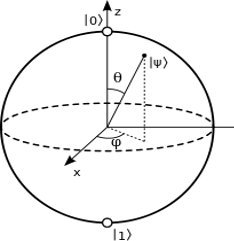
\includegraphics[width=0.4\textwidth]{figs/8.png}
\end{center} 
\end{frame}

\begin{frame} 
    \frametitle{量子比特的矩阵表示}
    \[\rs{\psi} =\alpha\rs{0}+\beta\rs{1} \] 
    态函数与系数矩阵有对应关系\\
   \[
    \begin{matrix} 
    \rs{\psi} =\begin{pmatrix}
            \alpha\\
            \beta
    \end{pmatrix}
    &    
    \rs{0} 
    =\begin{pmatrix}
        1\\
        0
    \end{pmatrix}
    &
    \rs{1} 
    =\begin{pmatrix}
        0\\
        1
    \end{pmatrix}
    \end{matrix}    
    \]
\end{frame}

\begin{frame} 
    \frametitle{量子比特的外积}
    由矩阵表示可知量子比特的外积$\rl{\psi}{\psi}$是一个$2\times 2$的矩阵,
    泡利矩阵是正交归一完全集,
    因此,外积可在泡利矩阵上展开!
    \[\begin{aligned}
    \rl{\psi}{\psi} 
    &=
    \begin{pmatrix}
        \alpha\\
        \beta
    \end{pmatrix}
    \begin{pmatrix}
        \alpha & \beta
    \end{pmatrix}
 \\
    &= \frac{1}{2}I +\frac{1}{2}\sin\theta\cos\varphi\sigma_x +\frac{1}{2}\sin\theta\sin\varphi\sigma_y+ \frac{1}{2}\cos\theta\sigma_z 
\end{aligned}\]
式中,泡利矩阵为
\[
\sigma_x =
\begin{pmatrix}
    0 & 1 \\
    1 & 0 
\end{pmatrix}, \qquad
\sigma_y =
\begin{pmatrix}
    0 & -i \\
    i & 0 
\end{pmatrix}, \qquad
\sigma_z =
\begin{pmatrix}
    1 & 0 \\
    0 & -1 
\end{pmatrix}
\]
\end{frame}

\section{4.双量子比特}


\begin{frame} 
\frametitle{双量子比特计算基矢态}
两个经典比特有四种状态:\\
00,01, 10, 11\\
(1).两个量子比特有四种计算基矢态:
\[\rs{00}, \qquad \rs{01}, \qquad \rs{01}, \qquad \rs{11} \] 
它们的矩阵表示由原矩阵的直积表示 
\[\rs{01} = \rs{0} \otimes \rs{1} =    
\begin{pmatrix}
    1\\
    0
\end{pmatrix}
\otimes
\begin{pmatrix}
    0\\
    1
\end{pmatrix}
=
\begin{pmatrix}
    1 \otimes \begin{pmatrix}
        0\\
        1
    \end{pmatrix}\\
    0 \otimes \begin{pmatrix}
        1\\
        0
    \end{pmatrix}
\end{pmatrix}
=
\begin{pmatrix}
    0\\
    1\\
    0\\
    0
\end{pmatrix}
 \] 

\end{frame}

\begin{frame} 
\[
\rs{00} = 
\begin{pmatrix}
    1\\
    0\\
    0\\
    0
\end{pmatrix},\qquad
\rs{01} = 
\begin{pmatrix}
    0\\
    1\\
    0\\
    0
\end{pmatrix},\qquad
\rs{10} = 
\begin{pmatrix}
    0\\
    0\\
    1\\
    0
\end{pmatrix},\qquad
\rs{1} = 
\begin{pmatrix}
    0\\
    0\\
    0\\
    1
\end{pmatrix}
\] \vspace{0.6em}
\Note 四个计算基矢态$ \rs{00}, \rs{01},\rs{10},\rs{11} $构成正交归一完全集。
\end{frame}

\begin{frame} 
    \frametitle{双量子比特叠加态}
(2). 双量子比特任意态是四个计算基矢态的叠加态:
 \[\rs{\psi} =\alpha_{00}\rs{00}+\alpha_{01}\rs{01}+\alpha_{10}\rs{10}+\alpha_{11}\rs{11}\]
 归一化条件:
 \[ \sum_{ij=0,1} |\alpha_{ij}|^2= 1\]
\end{frame}

\begin{frame} 
    \frametitle{测量后态函数}
\例[若对双量子比特的第一个位进行测量,设测量结果为$\rs{0}$,求测量后体系的状态]{}
 \[\rs{\psi} =\alpha_{00}\rs{00}+\alpha_{01}\rs{01}+\alpha_{10}\rs{10}+\alpha_{11}\rs{11}\]
 \解~测量导致后两计算基矢态消失,
 \[\rs{\psi} =\alpha_{00}\rs{00}+\alpha_{01}\rs{01}\]
 求归一化系数,得归一化态函数:
 \[\rs{\psi'} =\frac{\alpha_{00}\rs{00}+\alpha_{01}\rs{01}}{\sqrt{|\alpha_{00}|^2+ |\alpha_{01}|^2}} \]
\end{frame}

\begin{frame} 
    \frametitle{三量子比特}
(4).三量子比特有8个计算基矢态:\\
\[\rs{000}, \qquad \rs{001}, \qquad \rs{010}, \qquad \rs{011} , \qquad \rs{100}, \qquad \rs{101}, \qquad \rs{110}, \qquad \rs{111} \] 
三量子比特任意态是这8个计算基矢态的叠加态:
\[\rs{\psi} =\sum_{ijk=0,1} \alpha_{ijk}\rs{ijk}\] 
\end{frame}

\begin{frame} 
    \frametitle{n量子比特}
(5). n量子比特有$2^n$个计算基矢态:\\
{\Bullet} 当n=500时,计算基矢态的数目比宇宙中的原子数目还在多!\\
{\Bullet} 当n=100时,一台量子计算机可以完成全世界当前所有的计算任务!
\end{frame}

\section{4.量子逻辑门}

\begin{frame} 
    \frametitle{量子比特逻辑门}

{\Bullet} 量子计算由量子线路来完成信息的处理和传输,

{\Bullet} 量子线路主要由量子传输线和量子逻辑门构成,

{\Bullet} 量子逻辑门是进行逻辑运算的基本单元,

{\Bullet} 逻辑运算是一切数值计算的基础,

{\Bullet} 在数学上找到一套普适的量子逻辑门,可完成人类所有的逻辑运算。

{\Bullet} 在物理上实现普适的量子逻辑门,构造出量子计算机

\end{frame}

%\begin{frame}
    \includemedia[
    width=1.0\linewidth,height=0.60\linewidth, % 16:9
    activate=pageopen,
    addresource=figs/qubit.mp4,
    flashvars={
    source=figs/qubit.mp4
    &autoPlay=true % start playing on activation
    &loop=true
    }
    ]{}{VPlayer.swf}
%\end{frame}

\begin{frame}
    \frametitle{}
    \begin{tcolorbox3}[专题学术讨论-1]
        为什么经典计算机必将发展成为量子计算机?
    \end{tcolorbox3}
\end{frame}